\documentclass[13pt,a4paper]{article}
\usepackage[spanish,es-nodecimaldot]{babel}	% Utilizar español
\usepackage[utf8]{inputenc}					% Caracteres UTF-8
\usepackage{graphicx}						% Imagenes
\usepackage[hidelinks]{hyperref}			% Poner enlaces sin marcarlos en rojo
\usepackage{fancyhdr}						% Modificar encabezados y pies de pagina
\usepackage{float}							% Insertar figuras
\usepackage[textwidth=390pt]{geometry}		% Anchura de la pagina
\usepackage[nottoc]{tocbibind}				% Referencias (no incluir num pagina indice en Indice)
\usepackage{enumitem}						% Permitir enumerate con distintos simbolos
\usepackage[T1]{fontenc}					% Usar textsc en sections
\usepackage{amsmath}						% Símbolos matemáticos
\usepackage[ruled,vlined]{algorithm2e}      % Pseudocódigo
\usepackage{xcolor}
\usepackage{listings}
% Para que acepten tíldes los listing
\lstset{     
     literate=%
         {á}{{\'a}}1
         {é}{{\'e}}1
         {í}{{\'i}}1
         {ó}{{\'o}}1
         {ú}{{\'u}}1
         {Á}{{\'A}}1
         {É}{{\'E}}1
         {Í}{{\'I}}1
         {Ó}{{\'O}}1 
         {Ú}{{\'U}}1
         {ñ}{{\~n}}1 
         {Ñ}{{\~N}}1 
         {¿}{{?``}}1 
         {¡}{{!``}}1
}
\usepackage{dsfont}

% ==============================================================================

\usepackage{caption, subcaption}
\usepackage[section]{placeins}
\makeatletter
\def\fps@figure{H}
\makeatother

\usepackage{booktabs}
\usepackage{longtable}
\usepackage{array}
\usepackage{multirow}
\usepackage{wrapfig}
\usepackage{colortbl}
\usepackage{pdflscape}
\usepackage{tabu}
\usepackage{threeparttable}
\usepackage{threeparttablex}
\usepackage[normalem]{ulem}
\usepackage{makecell}
\usepackage{xcolor}
\usepackage[bottom]{footmisc}

\makeatletter
\newcommand*{\centerfloat}{%
  \parindent \z@
  \leftskip \z@ \@plus 1fil \@minus \textwidth
  \rightskip\leftskip
  \parfillskip \z@skip}
\makeatother

% ==============================================================================
% ==============================================================================

% Comando para poner el nombre de la asignatura
\newcommand{\asignatura}{Aplicaciones de Ciencia de Datos y Tecnologías Inteligentes}
\newcommand{\autor}{Ignacio Vellido Expósito}
\newcommand{\email}{ignaciove@correo.ugr.es}
\newcommand{\titulo}{Señales e imágenes biomédicas}
\newcommand{\subtitulo}{Anthropological Facial Approximation in Three Dimensions}

% Configuracion de encabezados y pies de pagina
\pagestyle{fancy}
\lhead{\autor{}}
\rhead{\asignatura{}}
\lfoot{Máster Ciencia de Datos e Ingeniería de Computadores}
\cfoot{}
\rfoot{\thepage}
\renewcommand{\headrulewidth}{0.4pt}		% Linea cabeza de pagina
\renewcommand{\footrulewidth}{0.4pt}		% Linea pie de pagina

% ==============================================================================
% ==============================================================================

% El objetivo, como os decía en clase, es elaborar un informe (como máximo de 3 páginas, que me enviarás en PDF), en donde resumas, de forma ordenada, clara y bien estructurada, las principales ideas del artículo. En concreto, el informe/resumen debe contener, al menos, la siguiente información:
% - qué problema se pretende resolver y por qué es importante resolverlo.
% - qué propone el artículo para resolver el problema.
% - ventajas y limitaciones de la aproximación propuesta, en comparación con métodos alternativos (si los hay).
% - qué resultados proporciona (a nivel cualitativo y cuantitativo).
% - breve comentario sobre vuestra opinión sobre el paper (relevancia de la materia, calidad y claridad de la escritura, rigor científico de la propuesta).

% La idea es que os expreséis con vuestras propias palabras y no copiéis el artículo literalmente. Evidentemente, podéis reforzar vuestros razonamientos y opiniones en base al artículo, citando fragmentos concretos, pero me gustaría ver en el texto que realmente entendisteis lo que leísteis y que os expresáis con claridad. De hecho, no dudéis en dejar claro aquello que no entendéis, porque es posible que algún artículo, en algún aspecto, resulte confuso o incluso contenga algún error. Valoraré, principalmente, la claridad de las ideas y la transferencia útil del conocimiento. Desde este punto de vista, no valoraré la cantidad sino la calidad: independientemente de la longitud del trabajo (siempre que respete el máximo de 3 páginas), si el contenido es adecuado (bien escrito y organizado, exposición clara, mostrando una buena comprensión de los elementos clave del artículo) lo calificaré con la máxima nota.

% Si no recuerdo mal, tenéis hasta el 20 de Junio para entregar los trabajos. En mi caso, no tendré problema en revisarlos y calificarlos con anterioridad a esa fecha. De hecho, mi intención es que, quien lo desee, puede enviarme el trabajo en los próximos días/semanas, y yo se lo puedo enviar, en caso de que sea necesario, corregido y con ideas para su mejora. De este modo, tendríais incluso la oportunidad de incorporar estas modificaciones/ideas y entregármelo de nuevo revisado. 

\begin{document}
    \pagenumbering{gobble}
    % ==============================================================================
% Pagina de titulo
\begin{titlepage}
    \begin{minipage}{\textwidth}
        \centering

        
\includegraphics[scale=0.5]{img/ugr.png}\\

        \textsc{\Large \asignatura{}\\[0.2cm]}
        \textsc{MÁSTER CIENCIA DE DATOS E INGENIERÍA DE COMPUTADORES}\\[1cm]

        \noindent\rule[-1ex]{\textwidth}{1pt}\\[1.5ex]
        \textsc{{\Huge \titulo\\[0.5ex]}}
        \textsc{{\Large \subtitulo\\}}
        \noindent\rule[-1ex]{\textwidth}{2pt}\\[2.5ex]

        \end{minipage}

        \vspace{0.3cm}

        \begin{minipage}{\textwidth}

        \centering

        \textbf{Autor}\\ {\autor{} \\ ignaciove@correo.ugr.es}\\[1.5ex]
        \vspace{0.4cm}

        
\includegraphics[scale=0.3]{img/etsiit.jpeg}
        
\includegraphics[scale=0.6]{img/master.png}

        \vspace{0.7cm}
        \textsc{Escuela Técnica Superior de Ingenierías Informática y de Telecomunicación}\\
        \vspace{1cm}
        \textsc{Curso 2020-2021}
    \end{minipage}
\end{titlepage}
% ==============================================================================
    
    \pagenumbering{arabic}
    \tableofcontents
    \thispagestyle{empty}				% No usar estilo en la pagina de indice

    \newpage

    % ==============================================================================

    % \section{Resultados globales}

Orden usado en las técnicas:
Under/Oversampling > NoiseFiltering > Instance Selection

\begin{figure}[ht]
    \centerfloat
    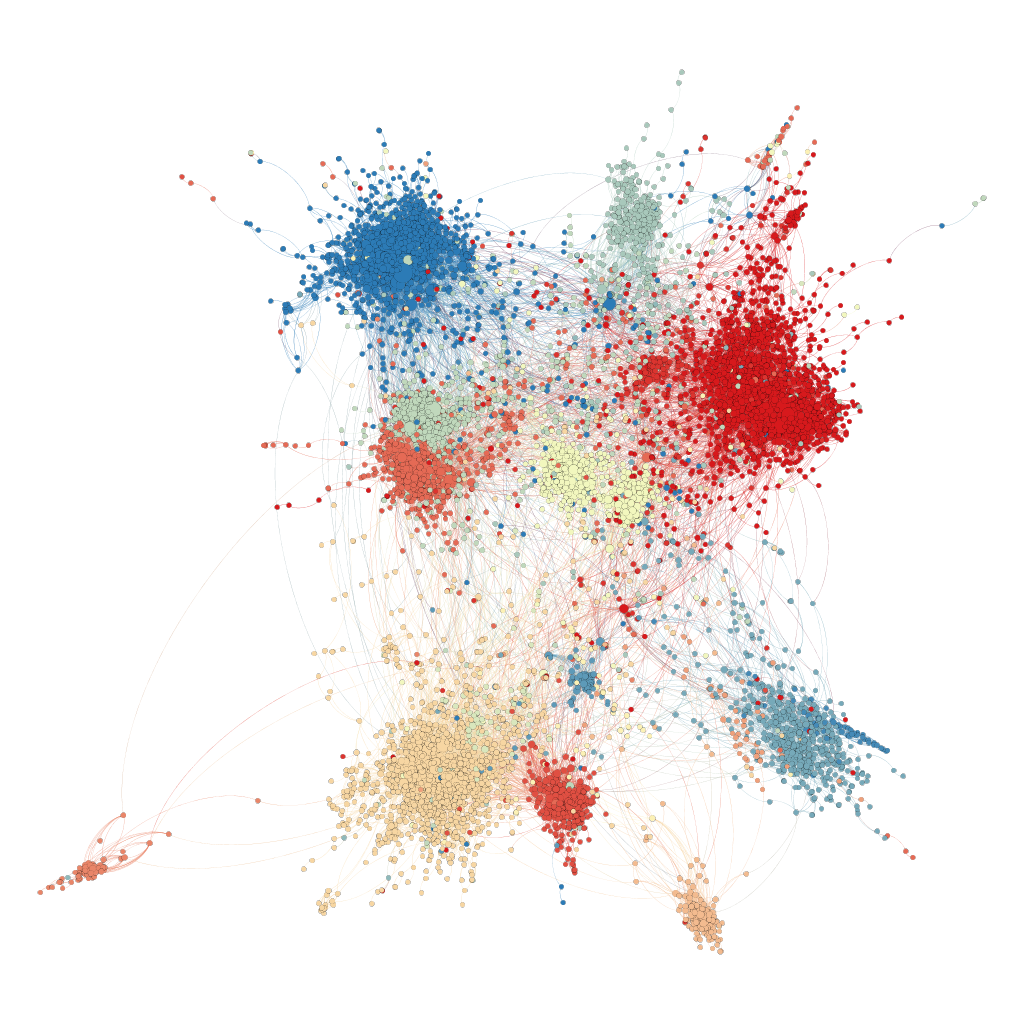
\includegraphics[width=1.097\textwidth]{img/resultados/grado-targets.png}
    \caption{Topología de la red. El color indica el país de cada usuario.}
\end{figure}

\begin{figure}[t]
    \centering
    \resizebox{0.78\columnwidth}{!}{%
    \begin{tabular}{| l | r |} 
        \hline
        \textbf{Medida} & \textbf{Valor} \\
        \Xhline{2\arrayrulewidth}
        Número de nodos \textbf{N} & 7,624 \\
        \hline
        Número de enlaces \textbf{L}	& 27,806 \\
        \hline
        Número máximo de enlaces \textbf{$L_{max}$} & 58117752 \\
        \hline
        Densidad del grafo \textbf{$L/L_{max}$} & 0.001 \\
        \Xhline{2\arrayrulewidth}
        Grado medio \textbf{<k>} & 7.294 \\
        \hline
        Diámetro \textbf{$d_{max}$} & 15 \\
        \hline
        Distancia media \textbf{d} & 5.232237269 \\
        \hline
        Coeficiente medio de clustering \textbf{<C>} & 0.285 \\
        \Xhline{2\arrayrulewidth}
        Número de componentes conexas & 1 \\
        \hline
        Número de nodos componente gigante (y \%) & 7,624 (100) \\
        \hline
        Número de aristas componente gigante (y \%) & 27,806 (100) \\
        \hline
    \end{tabular}
    }
    \caption{Medidas globales de la red.}
\end{figure} \newpage
\section{Descripción del problema}

\section{Propuesta}
Sistema holistic (que tiene en cuenta el conjunto de rasgos) para la estimación premortem (o post a partir de alguna imágen?) de una cara, gracias a un cráneo (o imágen ?) y un conjunto de landmarks indicados por un técnico forense ?

Para evaluar? uso 500 datos de diferentes rangos de edades y de ambos sexos.

También se proporciona el software públicamente para fomentar la colaboración y el progreso, un detalle que veo importante remarcar sobre la propuesta.

\section{Ventajas e inconvenientes}

\section{Resultados}

\section{Análisis}

\subsection{Sobre la relevancia}

% Intento valorar aquí la aportación \textbf{científica} de la propuesta, en contraposición con la labor de ingeniería del sistema construído (tengo esto en cuenta porque fue un detalle que me indicaron el la revisión de un paper). Por tanto, tenemos como aportaciones:

\subsection{Sobre la escritura}

% Cabe decir que existe mucha terminología del campo, que en mi caso se escapa de mis conocimientos. Aún así, esto se justifica al verse publicado en una revista forense, por lo que es de espera que su lectura por gente externa al "campo" no estuviera considerada.
% Pese a ello, no puedo negar que tras unas pocas lecturas las ideas y aportaciones principales quedan claras, sobre todo gracias a que el "jargon" se utiliza más en las figuras y tablas que el propio texto.

\subsection{Sobre el rigor científico en la propuesta (validación y evaluación)}

El artículo pretende justificar una aplicación genérica para aplicar la propuesta, pero al contar con datos únicamentes de Francia no lo afirma sino que lo sugiere como idea a evaluar. Esto me parece bastante correcto 

Los datos utilizados me parecen adecuados para el ámbito al que se dirige, ya que la obtención de datos es dificultosa ?

    % ==============================================================================

  %   \begin{figure}[ht]
  %     \centerfloat
  %     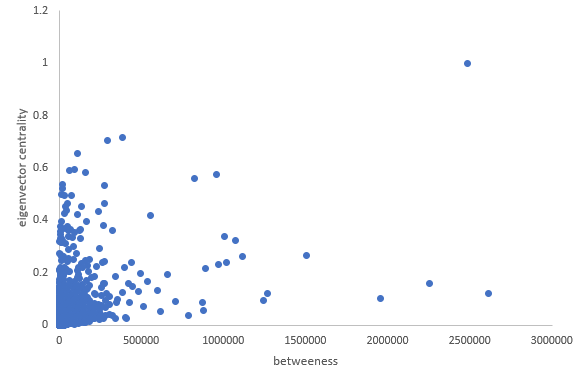
\includegraphics[width=0.75\textwidth]{img/resultados/betw-eig2.png}
  %     \caption{Relación intermediación-vector propio.}
  % \end{figure}

%   \begin{figure}[H]
%     \centering
%     \resizebox{0.9\columnwidth}{!}{%
%     \begin{tabular}{| l | l | l | l |} 
%         \hline
%         \textbf{Centralidad de Grado} & \textbf{Intermediación} & \textbf{Cercanía} & \textbf{Vector propio} \\
%         \Xhline{2\arrayrulewidth}
%         \textbf{7237} - 216 & 	\textbf{7199} - 2,612,617 & \textbf{7199} - 0.2907 & 	\textbf{7237} - 1.0000  \\
%         \hline
%         \textbf{3530} - 175 & 	\textbf{7237} - 2,486,453 & 	\textbf{7237} - 0.2856 & \textbf{3240} - 0.7149  \\
%         \hline
%         \textbf{4785} - 174 & 	\textbf{2854} - 2,253,302 & 	\textbf{4356} - 0.2816 & 	\textbf{3597} - 0.7052  \\
%         \hline
%         \textbf{524}   - 172 & 	\textbf{4356} - 1,953,690 & 	\textbf{2854} - 0.2803 & 	\textbf{763}   - 0.6555  \\
%         \hline
%         \textbf{3450} - 159 & \textbf{6101} - 1,504,994 & 	\textbf{5454} - 0.2798 & 	\textbf{2083} - 0.5940  \\
%         \hline
%     \end{tabular}
%     }
%     \caption{Tabla de actores más relevantes (identificador-valor).}
% \end{figure}

% \begin{figure}
%   \centering  
%   \begin{subfigure}[t]{0.48\textwidth}
%     \centering
%     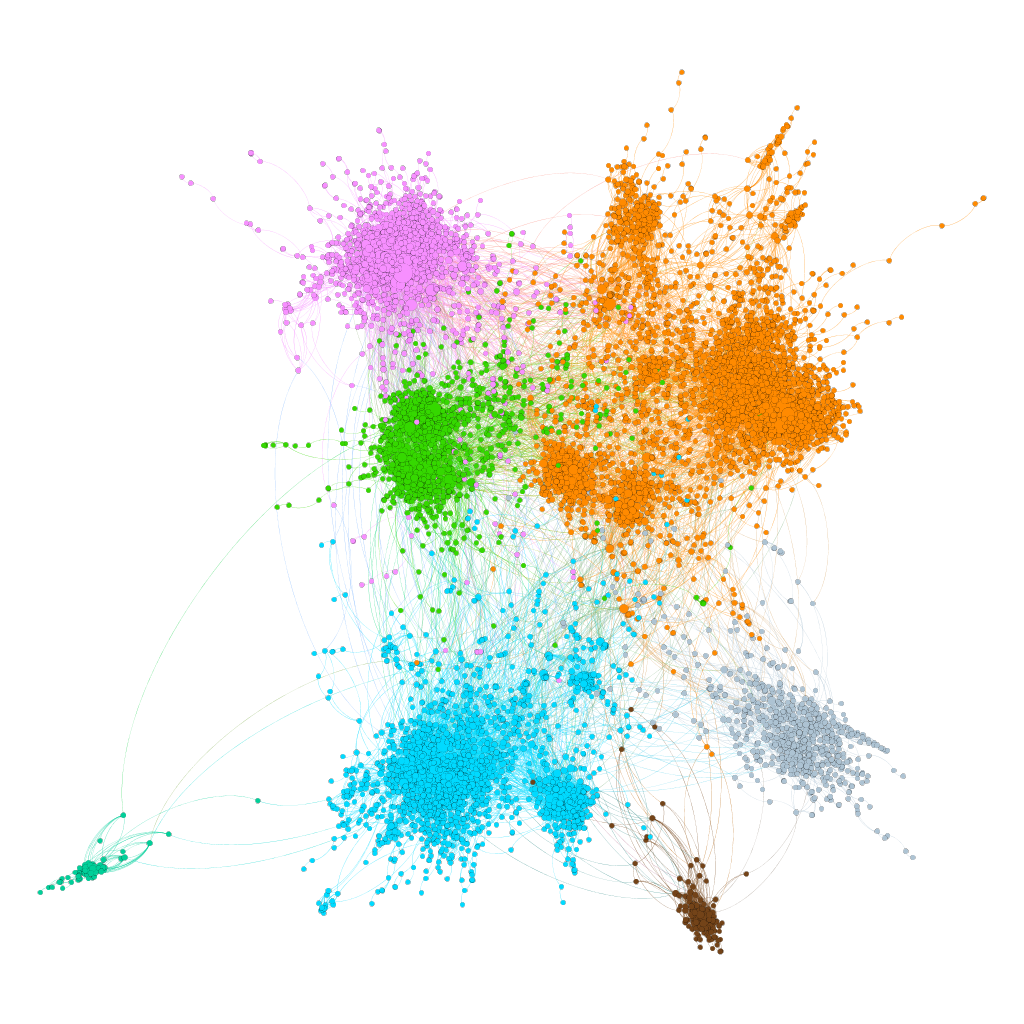
\includegraphics[width=\textwidth]{img/resultados/grado-leinen0.1.png}
%     \caption{Coeficiente 0.1.}
%   \end{subfigure}
%   \vspace{7mm}
%   \hfill
%   \begin{subfigure}[t]{0.48\textwidth}
%     \centering
%     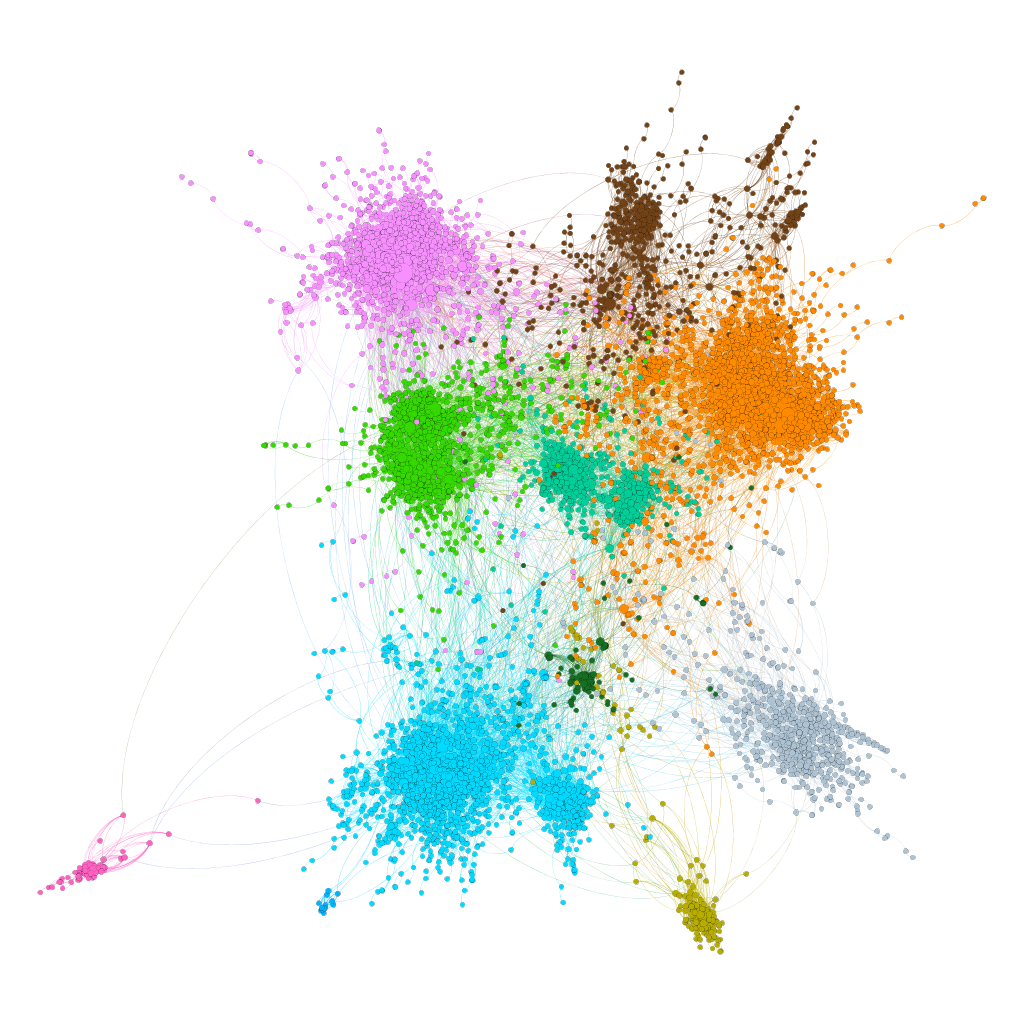
\includegraphics[width=\textwidth]{img/resultados/grado-leinen0.25.png}
%     \caption{Coeficiente 0.25.}
%   \end{subfigure}
%   \hfill
%   \begin{subfigure}[t]{0.48\textwidth}
%     \centering
%     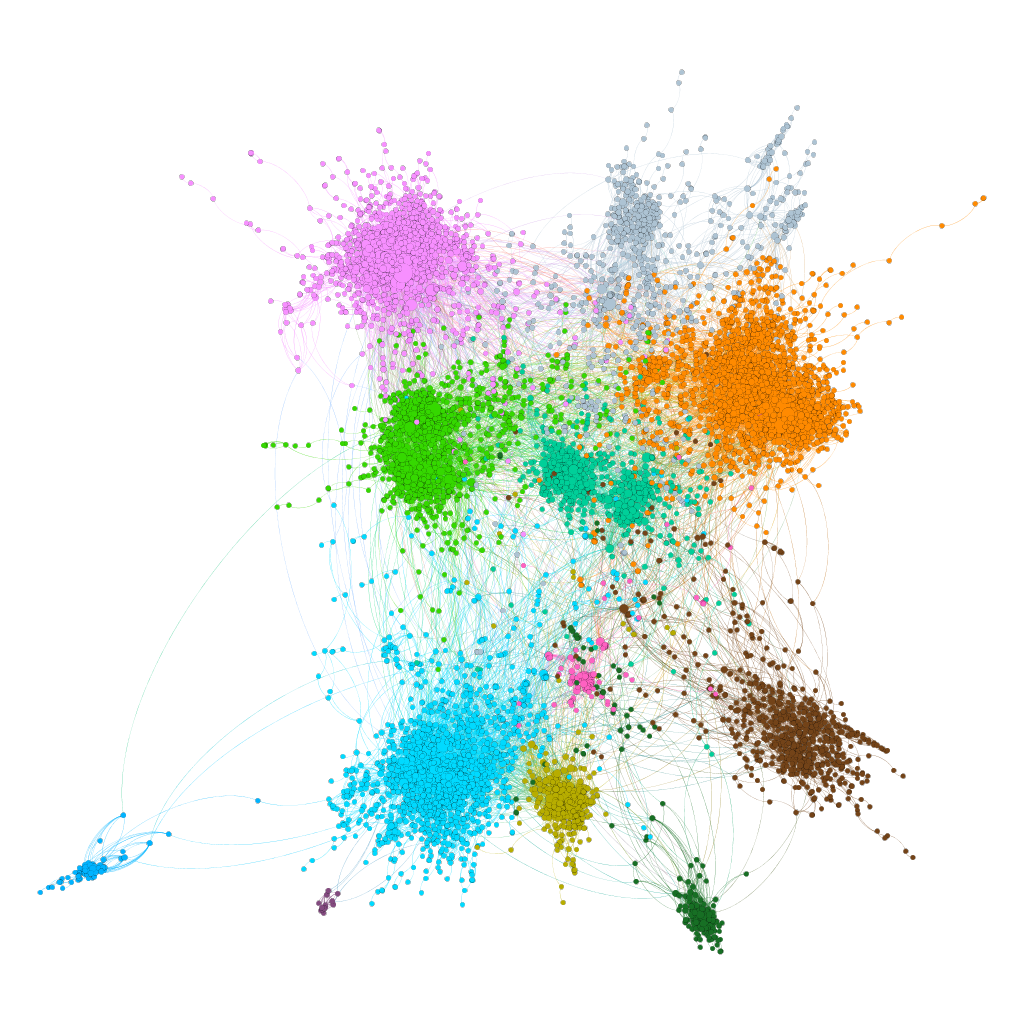
\includegraphics[width=\textwidth]{img/resultados/grado-leinen0.33.png}
%     \caption{Coeficiente 0.33.}
%   \end{subfigure}
%   \hfill
%   \begin{subfigure}[t]{0.48\textwidth}
%     \centering
%     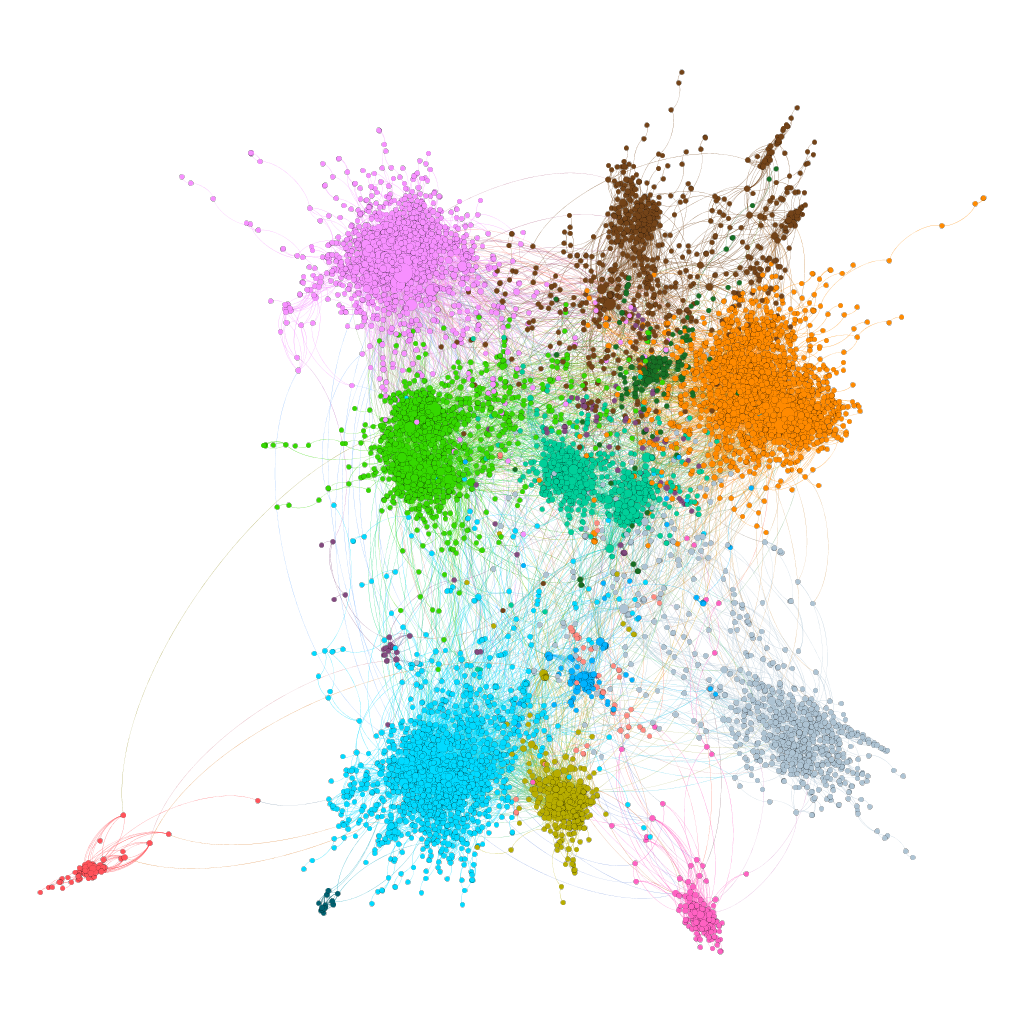
\includegraphics[width=\textwidth]{img/resultados/grado-leinen0.5.png}
%     \caption{Coeficiente 0.5.}
%   \end{subfigure}

%   \caption{Comunidades detectadas por el algoritmo Leinen para diferentes coeficientes.}
% \end{figure}

    \setlength{\parskip}{1em}
    \newpage
    % \nocite{*}
    % \bibliography{bibliografia}
  	% \bibliographystyle{plain}
\end{document}